\chapter{Evaluation}\label{chap:evaluation}
Through the use of the framework described in the previous chapter, we evaluate four different algorithms for next-activity prediction: Two implementations that mimic Evermann et al. and Schönig et al, and the previously presented PFS and SP2. In doing so, we will analyze the different approaches for structuring the training data for performance differences.

As we follow the KDD process, this chapter briefly leads through the data processing and transformation phases in \autoref{sec:eval:data-preprocessing} and \autoref{sec:eval:data-transformation}. The latter section also covers the strategy used to engineer the SP-2 and subsequence features. Then, the test setup and the used training strategy is presented in \autoref{sec:eval:test-setup}, followed by the set of criteria by which we judge the results in \autoref{sec:eval:criteria}. Finally, the chapter ends with the presentation and discussion of the results in \autoref{sec:eval:results}. Used and relevant technologies are highlighted in the respective sections.

\section{Data preprocessing}
\label{sec:eval:data-preprocessing}
In the first step of KDD process~\cite{fayyad1996data}, the data was preprocessed to eliminate generally known properties that hinder machine learning model performance. Here, this encompassed two steps for both datasets:

\begin{enumerate}
    \item All columns which exhibited zero entropy, i.e. which were constituted of a single value, were dropped.
    \item Features which correlated strongly were eliminated. To account for categorical correlation, the bias-corrected version of Cramér's~V~\cite{bergsma2013bias} was used.
\end{enumerate}


For both BPIC2011 and BPIC2012 datasets, the column \texttt{lifecycle:transition} was dropped in step 1. To make statements about upcoming workflow-related activities only, only completion events related to workflow activities were kept in the BPIC2012 log \cite{evermann2016}.

In step 2, the bi-directional results in \autoref{fig:bpic2011-correlation-heatmap} from Cramér's V revealed that the variables \texttt{Producer code}, \texttt{Activity code} and \texttt{Specialism code} correlate strongly with many others in the BPIC2011 dataset. Thus, these were dropped. As evidenced in \autoref{fig:bpic2012-correlation-heatmap}, the BPIC2012 dataset with its small number of features did not require any removals.

\begin{figure}
\centering
\subfloat[][BPIC2011 Cramér's V heatmap]{
    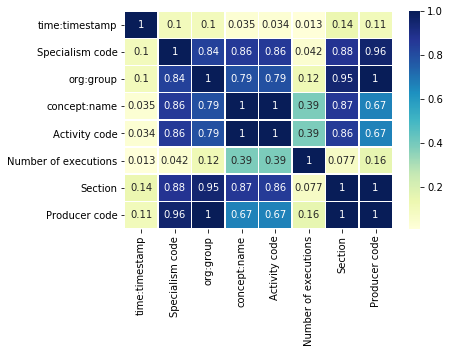
\includegraphics[width=0.7\textwidth]{gfx/bpic2011-correlation-matrix.png}
    \label{fig:bpic2011-correlation-heatmap}
}
\qquad
\subfloat[][BPIC2012 Cramér's V heatmap]{
    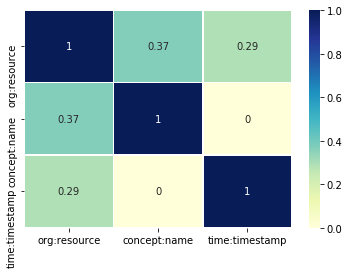
\includegraphics[width=0.7\textwidth]{gfx/bpic2012-correlation-matrix.png}
    \label{fig:bpic2012-correlation-heatmap}
}
\caption{Correlation heatmaps obtained from Cramér's~V.}
\end{figure}

The activities described above were conducted in JupyterLab notebooks~\cite{web:jupyter}, where Anaconda~\cite{web:anaconda} was used to create a stable development environment. The OpyenXes~\cite{web:opyenxes} library proved to be especially useful for parsing the raw XES logs from BPIC.

\section{Data transformation}
\label{sec:eval:data-transformation}
Having removed unneeded features, the remaining ones were encoded following standard practice. Each numerical feature $x$ was normalized for with values specific to each trace using the min-max method:

$$normalize(x) = \frac{x-min(x)}{max(x)-min(x)}$$

Categorical features without ordinal properties, which were all of them, were encoded using one-hot encoding if possible. In the case of the input for the Evermann model, they were encoded with dictionary encoding, as this is required for Embedding layers.

\subsection*{SP-2 feature engineering}
For every trace, SP-2 features mark whether an activity has occured yet. Thus, these features are engineered in an iterative fashion, as \autoref{lst:sp2-generation} outlines. For every trace, a new data frame \texttt{sp2\_df} is created and the occurence of the first activity is marked inside it. For all following activities, the contents of the previous row inside \texttt{sp2\_df} are copied into the current one and the presence of the current activity is marked. This repeats itself until the trace has been processed completely.

\begin{figure}
\begin{minted}
sp2_df = pd.DataFrame(columns=activity_labels, index=range(0,len(t)), dtype=np.bool)
for col in sp2_df.columns: sp2_df[col].values[:] = 0
  sp2_df["{0}{1}".format(sp2_prefix,
                          t["concept:name"][0])].values[0]  = 1

  for i in range(1,len(t)):
    first_activity_name = t["concept:name"].iloc[i]
    col = "{0}{1}".format(sp2_prefix,first_activity_name)
  
    sp2_df.values[i] = sp2_df.values[i-1]
    sp2_df[col].values[i] = 1
\end{minted}
\caption{exemplary listing}
\label{lst:sp2-generation}
\end{figure}

\subsection*{Sub-sequence feature engineering}
The sub-sequence features for the PFS model were created with the help of the \textit{prefixspan-py} library~\cite{web:prefixspan-py}. As \autoref{lst:pfs-mining} shows, the library greatly facilitates obtaining closed sequences ranked by support and returns a two-dimensional array of sub-sequences, containing one array per sub-sequence.

\begin{figure}
\begin{minted}{python}
prefixspan_traces = PrefixSpan(encoded_traces)
closed_sequences = prefixspan_traces.topk(25, closed=True)
\end{minted}
\caption{Obtaining closed sequences using the \textit{prefixspan-py} library.}
\label{lst:pfs-mining}
\end{figure}

\todo[inline]{This has to be rewritten, the algorithm is wrong}
After mining the sequences, a loop is executed for every trace, shown in \autoref{lst:subsequence-feature-creation}. The activity at the current index is compared with the beginning of every subsequence in the list of subsequences. If they are equal, the foremost activity of that subsequence is popped. Should this deplete the list, the subsequence is considered as occurred and is marked as such in the feature vector. This continues until the end of every trace.

\section{Test setup}
\label{sec:eval:test-setup}
To conduct the experiments, Docker containers were built with the Anaconda environment inside them~\cite{web:docker}. Using a version of Docker for GPU applications running on NVIDIA hardware~\cite{web:nvidia-docker}, each network-formatting combination was trained and evaluated on a single NVIDIA K80 GPU of the HPI FutureSOC Lab~\cite{web:fsoc}. The complete source code is available on GitHub via \href{https://github.com/flxw/master-thesis-code}{flxw/master-thesis-code}.\\

Each model was saved when its validation loss hit a new record low. If the validation loss did not change for 10 epochs, the training was interrupted, also called \textit{early stopping}. \autoref{tab:network-info} illustrates information about the training setup of the networks side-by-side. As Evermann et al. made use of a version of Tensorflow that is deprecated by now, our implementation in Keras can only be understood as an approximation. Their "unrolled LSTM" can not be implemented in the same way in Keras.

\begin{table}[ht!]
    \centering
    \begin{tabular}{lcccc}
        \textbf{Network} & Evermann & Schönig & SP2 & PFS\\
        \hline
        \textbf{Optimizer} & SGD\footnote{SGD stands for Stochastic Gradient Descent. Additionally setting the learning rate decay to $0.75$ at the $25^{th}$ epoch.} & RMSprop  & RMSprop & RMSprop\\
        \textbf{Loss}    & & & &\\
        \textbf{Epochs}  & 50 & 100 & 100 & 100\\
        \textbf{BPIC2011 features} & 1 & 655 & 655 + 625 & 655 + 25 \\
        \textbf{BPIC2012 features} & 1 & 655 & 655 + 625 & 655 + 25 \\
    \end{tabular}
    \caption{Used hyper-parameters for each approach, the left two columns as chosen by the authors. The number of epochs is to be understood as the maximum number of epochs, as training may stop early.}
    \label{tab:network-info}
\end{table}
\todo[inline]{similar table for formatters}
\todo[inline]{K-Fold, pattern implementation}

\section{Evaluation criteria}
\label{sec:eval:criteria}
Three metrics of the four aforementioned implementations shall be the focus of the evaluation of the results:

\begin{enumerate}
    \item\textbf{Accuracy} - The share of correct next-activity predictions.
    \item\textbf{Earliness} - Whether and how early the prediction accuracy begins to stabilize as the trace progresses; see Francescomarino~\cite{francescomarino2015}.
    \item\textbf{Resource consumption} - The amount of time and memory required during training.
\end{enumerate}

While the first two criteria target the usability of the results, the last one permits making a judgment about the usefulness of the added features. This allows making a more informed decision about the necessity of the increased resource consumption.

\section{Results}
\label{sec:eval:results}


\subsection*{Accuracy}
\subsection*{Earliness}
\subsection*{Resource consumption}

